% 
% Assignment 1 for Image Processing.
% Timothy van der Valk.
% 2336715.
%

% Preamble {{{1
\documentclass[10pt, a4paper]{article}
\usepackage{geometry}
\usepackage{graphicx}
\usepackage{array}
\usepackage{tabularx}
\usepackage{caption}
\usepackage{float}
\usepackage{xfrac}

\usepackage{pgfplots}
\pgfplotsset{compat=1.18}

\setlength{\parindent}{0pt}
\setlength{\tabcolsep}{2pt}

\newcommand{\imagecell}[2]{%
	\begin{minipage}[t]{\linewidth}
		\centering
		\includegraphics[
		height=30mm,
		keepaspectratio
		]{#1}\\
		{\scriptsize #2}
	\end{minipage}%
}

\title{Image Processing\\Assignment 1}
\author{Timothy van der Valk\\2336715}

\begin{document}
\maketitle

\section*{Task 1 | Edge Detection} %{{{1
%{{{2

I have implemented an edge detection pipeline consisting of the following steps:
\begin{enumerate}
	\item Apply a Gaussian or Median filter. For Gaussians, we used $\sigma=(k-1)/5$ as recommended 
		by the book \cite[p.~114]{texbook}, where $k$ is the kernel size.
	\item Apply the edge magnitude filter using Sobel kernels. The magnitudes were
		normalized based on the largest value, because otherwise the image would get too dark
		and not be visible after thresholding.
	\item Apply thresholding from pixel intensity 75. This value has been chosen because
		it resulted in the most performant and consistent results for all kernel sizes.
\end{enumerate}

\subsection*{Analysis for Low-Noise Images}
The results for a clean tram image can be seen in Table \ref{task1_clean}.
The Median filter performs best on the smaller kernel, where it can remove small structures
that are irrelevant to edge detection. As the kernel size grows, the Median filter quickly
flattens many important surfaces, leaving only a few main edges visible after thresholding.
The Gaussian in comparison performs far better but becomes thicker due to our increasing value for $\sigma$.

\subsection*{Analysis for High-Noise Images}
The results for a noisy tram image can be seen in Table \ref{task1_noisy}.
In this case, it is clear that the Gaussian kernel is far worse for smaller kernels.
This is caused by its inability to remove strong, small noise effectively when the noise is
allowed to dominate a small amount of samples. The Median filter performs as expected
by efficiently removing small structures of noise. However, it suffers from the same problem
as before, where it flattens surfaces to the same brightness.
This causes a majority of the edges to be lost.

\pagebreak

\newgeometry{
    left=8mm,
    right=8mm,
    top=15mm,
    bottom=8mm
}

\begin{figure}[H] % Clean images {{{2
	\centering
	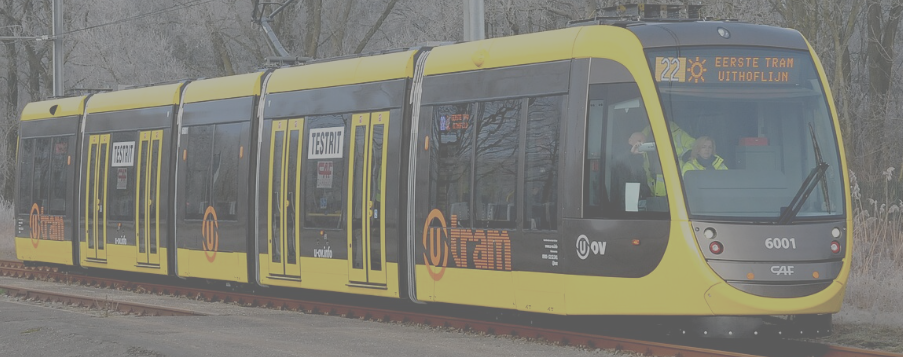
\includegraphics[width=80mm]{results/image_for_tasks1and2.png}\\
	{\scriptsize Reference image.}
	\vspace{5mm}

	\begin{tabularx}{\textwidth}{XX}

		% 3x3
		\imagecell{results/task1/clean\_gaussian3.png}{Gaussian 3x3 with $\sigma=0.4$.}
		&
		\imagecell{results/task1/clean\_median3.png}{Median 3x3.}
		\\[1cm]

		% 7x7
		\imagecell{results/task1/clean\_gaussian7.png}{Gaussian 7x7 with $\sigma=1.2$.}
		&
		\imagecell{results/task1/clean\_median7.png}{Median 7x7.}
		\\[1cm]

		% 11x11
		\imagecell{results/task1/clean\_gaussian11.png}{Gaussian 11x11 with $\sigma=2$.}
		&
		\imagecell{results/task1/clean\_median11.png}{Median 11x11.}
		\\[1cm]

		% 15x15
		\imagecell{results/task1/clean\_gaussian15.png}{Gaussian 15x15 with $\sigma=2.8$.}
		&
		\imagecell{results/task1/clean\_median15.png}{Median 15x15.}
		\\[1cm]

		% 19x19
		\imagecell{results/task1/clean\_gaussian19.png}{Gaussian 19x19 with $\sigma=3.6$.}
		&
		\imagecell{results/task1/clean\_median19.png}{Median 19x19.}
	\end{tabularx}
	\captionof{table}{
	Edge detection pipeline applied to clean tram images.}
	\label{task1_clean}
\end{figure}

\begin{figure}[H] % Noisy images {{{2
	\centering
	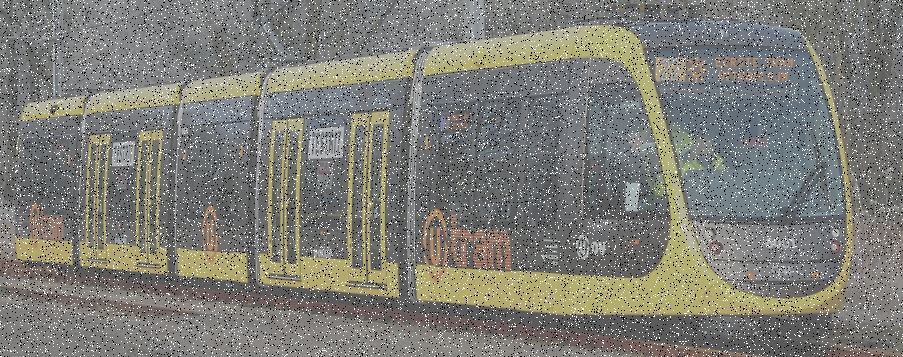
\includegraphics[width=80mm]{results/image_for_task1_noisy.png}\\
	{\scriptsize Reference image.}
	\vspace{5mm}

	\begin{tabularx}{\textwidth}{XX}

		% 3x3
		\imagecell{results/task1/noisy\_gaussian3.png}{Gaussian 3x3 with $\sigma=0.4$.}
		&
		\imagecell{results/task1/noisy\_median3.png}{Median 3x3.}
		\\[1cm]

		% 7x7
		\imagecell{results/task1/noisy\_gaussian7.png}{Gaussian 7x7 with $\sigma=1.2$.}
		&
		\imagecell{results/task1/noisy\_median7.png}{Median 7x7.}
		\\[1cm]

		% 11x11
		\imagecell{results/task1/noisy\_gaussian11.png}{Gaussian 11x11 with $\sigma=2$.}
		&
		\imagecell{results/task1/noisy\_median11.png}{Median 11x11.}
		\\[1cm]

		% 15x15
		\imagecell{results/task1/noisy\_gaussian15.png}{Gaussian 15x15 with $\sigma=2.8$.}
		&
		\imagecell{results/task1/noisy\_median15.png}{Median 15x15.}
		\\[1cm]

		% 19x19
		\imagecell{results/task1/noisy\_gaussian19.png}{Gaussian 19x19 with $\sigma=3.6$.}
		&
		\imagecell{results/task1/noisy\_median19.png}{Median 19x19.}
	\end{tabularx}
	\captionof{table}{Edge detection pipeline applied to noisy tram images.}
	\label{task1_noisy}
\end{figure}

\restoregeometry

\section*{Task 2 | Grayscale Erosion} %{{{1
%{{{2
I applied Grayscale Erosion to the tram images with increasing kernel sizes. 
The square structuring elements had a constant value of $0$.

\subsection*{Analysis}

The effect of Grayscale Erosion with a zero kernel comes down to taking the minimum
of the neighborhood around a pixel. This can be observed by the fact that there are
square patterns forming around pixels of lowest intensity. See Table \ref{task2_erosion}.\\[2mm]
It can be expected that as the minimization-kernel increases in size,
the number of unique pixel intensities drop as they become the same as the local minimum.
This in turn also causes a decrease in average intensity. These trends can be seen in Figure \ref{task2_plot}.

%{{{2 Plot
\begin{figure}[H]
    \centering
	\begin{minipage}{0.495\textwidth}
		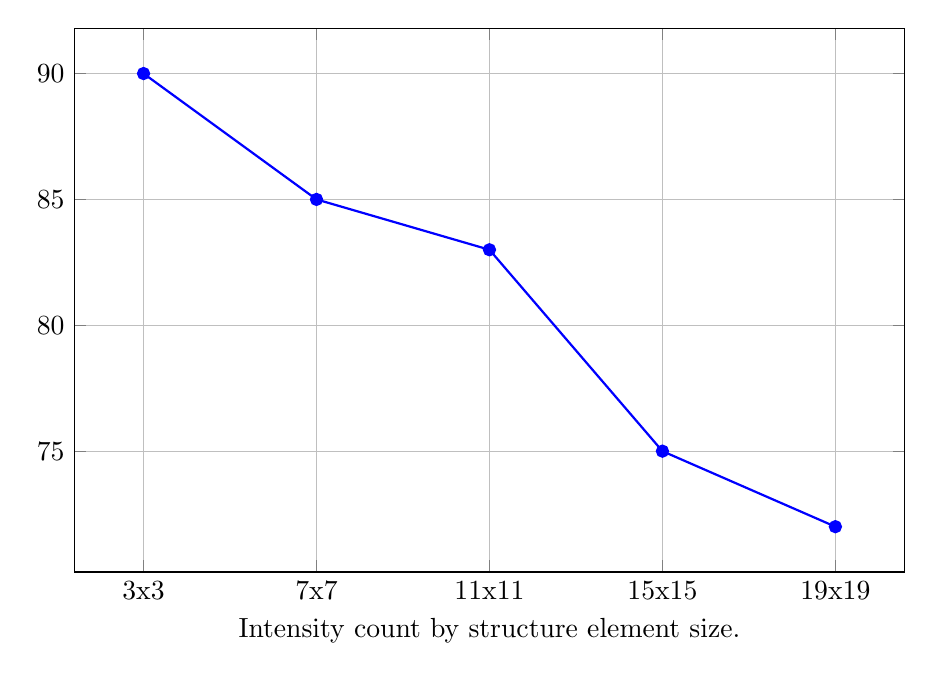
\begin{tikzpicture}
			\begin{axis}[
				width=\textwidth,
				height=0.7\textwidth,
				xlabel={Intensity count by structure element size.},
				xtick={1,2,3,4,5},
				xticklabels={3x3,7x7,11x11,15x15,19x19},
				grid=major,
			]

			% Number of unique intensities
			\addplot[
				mark=*,
				thick,
				color=blue
			] coordinates {
				(1,90)
				(2,85)
				(3,83)
				(4,75)
				(5,72)
			};
			\end{axis}
		\end{tikzpicture}
	\end{minipage}
	\hfill
	\begin{minipage}{0.495\textwidth}
		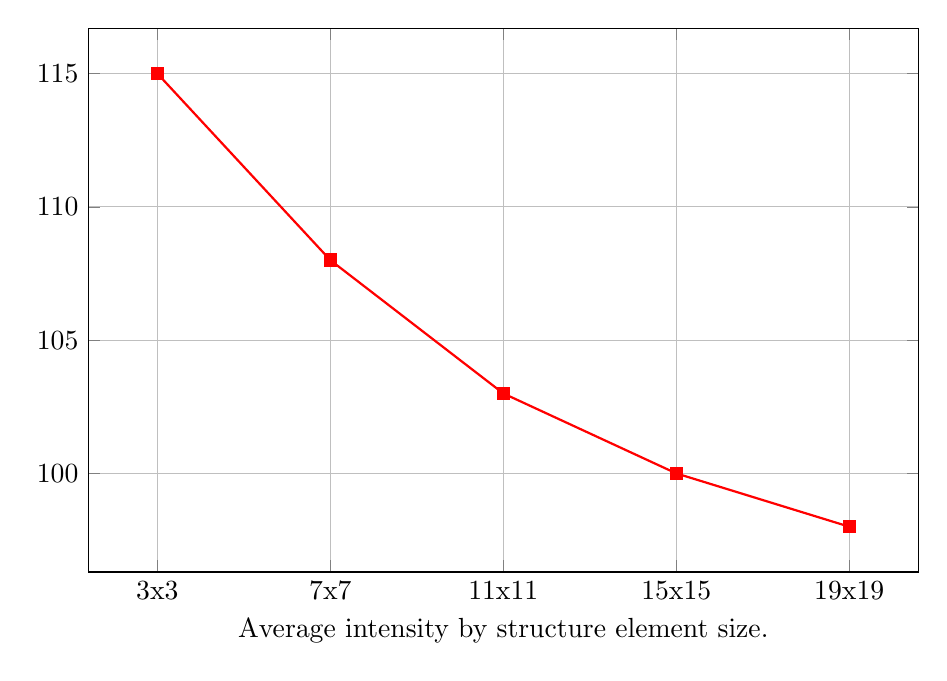
\begin{tikzpicture}
			\begin{axis}[
				width=\textwidth,
				height=0.7\textwidth,
				xlabel={Average intensity by structure element size.},
				xtick={1,2,3,4,5},
				xticklabels={3x3,7x7,11x11,15x15,19x19},
				grid=major,
			]

			% Average intensity
			\addplot[
				mark=square*,
				thick,
				color=red
				] coordinates {
					(1,115)
					(2,108)
					(3,103)
					(4,100)
					(5,98)
				};
        	\end{axis}
	    \end{tikzpicture}
	\end{minipage}

    \caption{Plot of the number of unique intensities (left) and the average pixel intensity (right) of
	Grayscale Erosion applied with increasing structure element sizes.}
    \label{task2_plot}
\end{figure}

\pagebreak

% Images {{{2
\newgeometry{
    left=8mm,
    right=8mm,
    top=15mm,
    bottom=8mm
}

\begin{figure}[H] 
	\begin{tabularx}{\textwidth}{X}
		% Reference.
		\imagecell{results/image\_for\_tasks1and2.png}{Reference Image.}
		\\[1cm]

		% 3x3
		\imagecell{results/task2/erosion3.png}{Grayscale Erosion with a flat 3x3 element.}
		\\[1cm]

		% 7x7
		\imagecell{results/task2/erosion7.png}{Grayscale Erosion with a flat 7x7 element.}
		\\[1cm]

		% 11x11
		\imagecell{results/task2/erosion11.png}{Grayscale Erosion with a flat 11x11 element.}
		\\[1cm]

		% 15x15
		\imagecell{results/task2/erosion15.png}{Grayscale Erosion with a flat 15x15 element.}
		\\[1cm]

		% 19x19
		\imagecell{results/task2/erosion19.png}{Grayscale Erosion with a flat 19x19 element.}
	\end{tabularx}
	\captionof{table}{
	Grayscale Erosion pipeline applied to tram images.}
	\label{task2_erosion}
\end{figure}

\restoregeometry
\pagebreak
\section*{Task 3 | Binary Closing} %{{{1

I have implemented Binary Closing with white pixels representing foreground.
The structure elements are squares with all values set to true.

\subsection*{Analysis}

The effect of Binary Closing is to first perform a Dilation, followed by an Erosion.
This causes holes and gaps between white pixels to close up if they are smaller than
twice the structure size. See Table \ref{task3_closing}. This effect can be seen in the 3x3 image, for example, where the
black dot in the top left is closed up by the surrounding white pixels.
For the larger structure sizes, we see that gaps between large blocks are closed up
for the 7x7 element, and that the large black square on the bottom right is eliminated in 11x11.\\[2mm]
Therefore, we would expect that the number of white foreground pixels increases when we
use larger structure sizes. This effect can be seen in Figure \ref{task3_plot}.
\begin{figure}[H] %{{{2
    \centering
	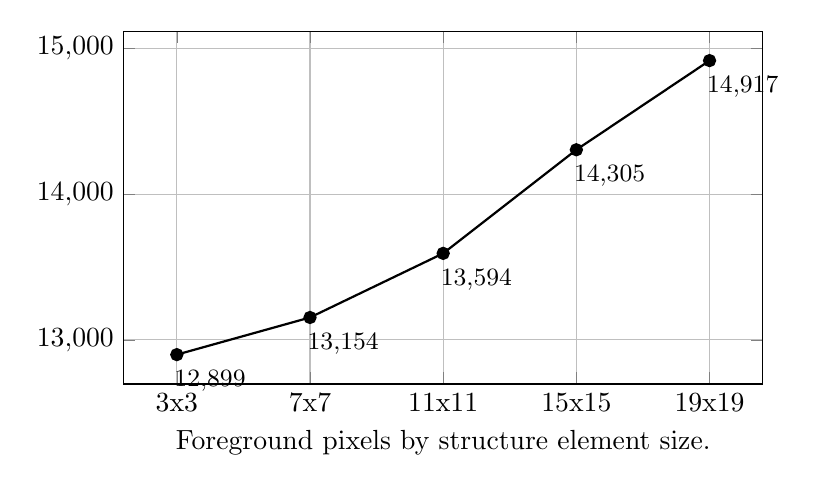
\begin{tikzpicture}
		\begin{axis}[
			width=0.8\textwidth,
			height=0.5\textwidth,
			xlabel={Foreground pixels by structure element size.},
			xtick={1,2,3,4,5},
			xticklabels={3x3,7x7,11x11,15x15,19x19},
			grid=major,
			scaled y ticks=false,
			nodes near coords,
			nodes near coords align={vertical},
			every node near coord/.append style={
				xshift=12pt,
				yshift=-17pt,
				font=\small
			},
		]

		% Number of unique intensities
		\addplot[
			mark=*,
			thick,
		] coordinates {
			(1,12899)
			(2,13154)
			(3,13594)
			(4,14305)
			(5,14917)
		};
		\end{axis}
	\end{tikzpicture}
    \caption{Plot of the number of foreground pixels after applying Binary Closing.}
    \label{task3_plot}
\end{figure}

\pagebreak

% Images {{{2
\newgeometry{
    left=8mm,
    right=8mm,
    top=15mm,
    bottom=8mm
}

\begin{figure}[H] 
	\begin{tabularx}{\textwidth}{X}
		% Reference.
		\imagecell{results/image\_for\_task3.png}{Reference Image.}
		\\[1cm]

		% 3x3
		\imagecell{results/task3/closing3.png}{Binary Closing with a flat 3x3 element.}
		\\[1cm]

		% 7x7
		\imagecell{results/task3/closing7.png}{Binary Closing with a flat 7x7 element.}
		\\[1cm]

		% 11x11
		\imagecell{results/task3/closing11.png}{Binary Closing with a flat 11x11 element.}
		\\[1cm]

		% 15x15
		\imagecell{results/task3/closing15.png}{Binary Closing with a flat 15x15 element.}
		\\[1cm]

		% 19x19
		\imagecell{results/task3/closing19.png}{Binary Closing with a flat 19x19 element.}
	\end{tabularx}
	\captionof{table}{
	Binary Closing pipeline applied to test images.}
	\label{task3_closing}
\end{figure}

\restoregeometry
\pagebreak
\begin{thebibliography}{9} %{{{1
\bibitem{texbook}
Principles of Digital Image Processing: Fundamental Techniques, Wilhelm Burger, Mark J. Burge. Springer 2009.
\end{thebibliography}

\end{document}
